%&"../virtual"

\begin{document}
    \title{Libvirt}
    \maketitle
    \tableofcontents

    \section{要求}
    Install Libvirt, then write python or C script with Libvirt Python or C API to get virtual machine ID, name, max memory, and the number of virtual CPUs.
    
    \section{编译并安装 libvirt}

    改良教程\cite{libvirt}的方法,安装 Ubuntu 版本的依赖包,下载 libvirt 4.10.0 源文件配置(如图 \ref{fig:configurelibvirt})并编译(如图 \ref{fig:makelibvirt})。

    \code[language=bash]{INSTALL.sh}

    \begin{figure}[H]
        \centering
        \begin{minipage}{0.48\textwidth}
            \centering
            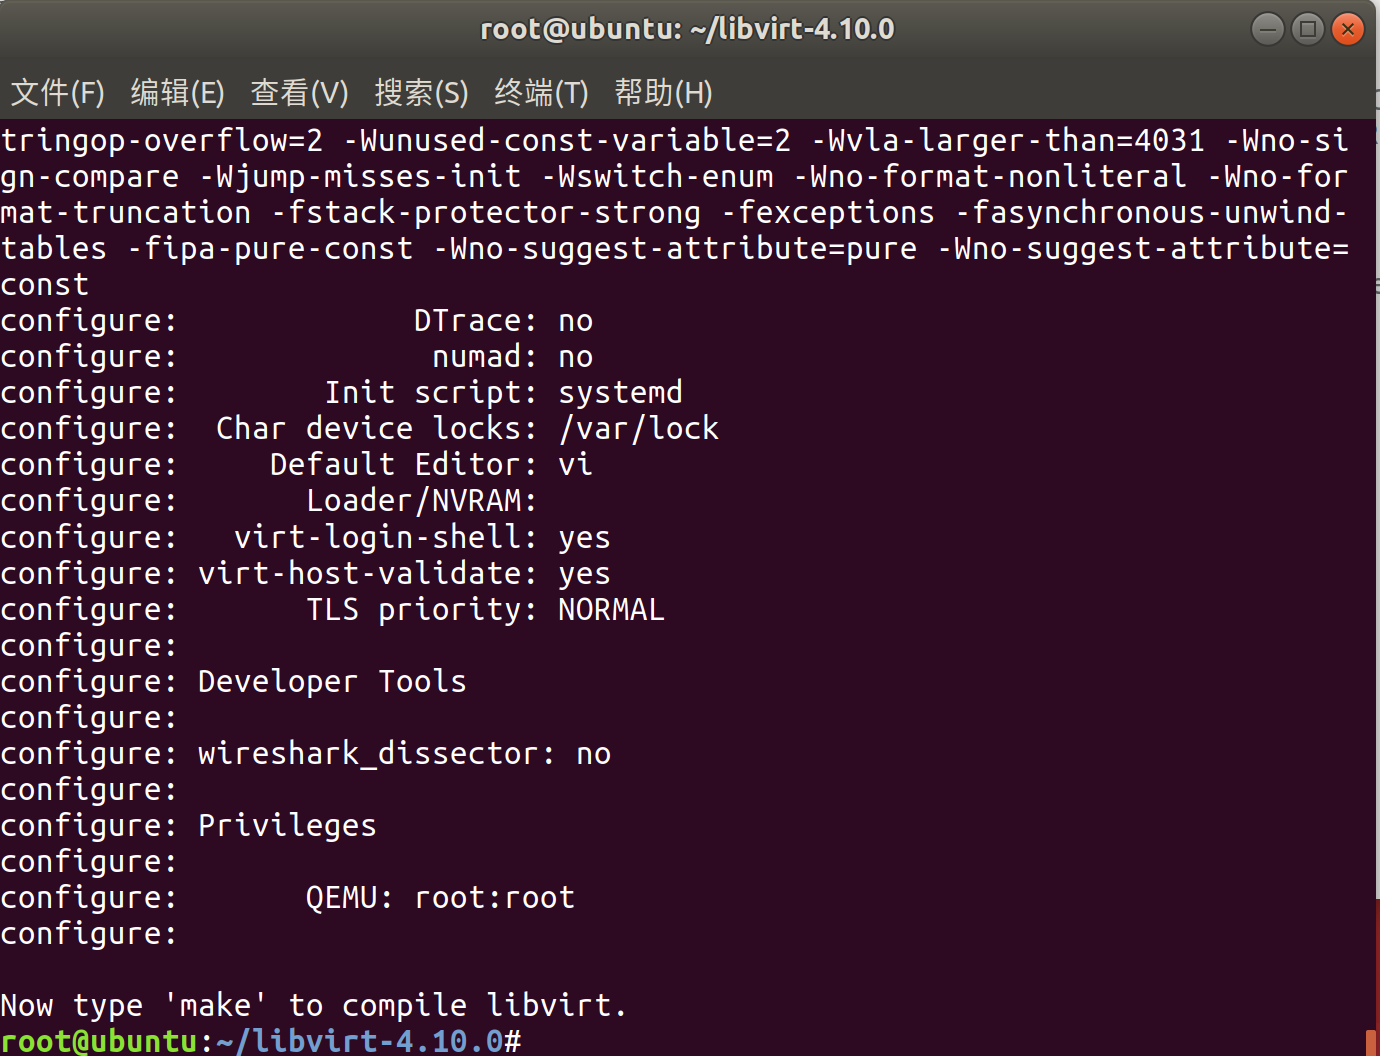
\includegraphics[width=\linewidth]{configurelibvirt}
            \caption{配置 libvirt}\label{fig:configurelibvirt}
        \end{minipage}
        \begin{minipage}{0.48\textwidth}
            \centering
            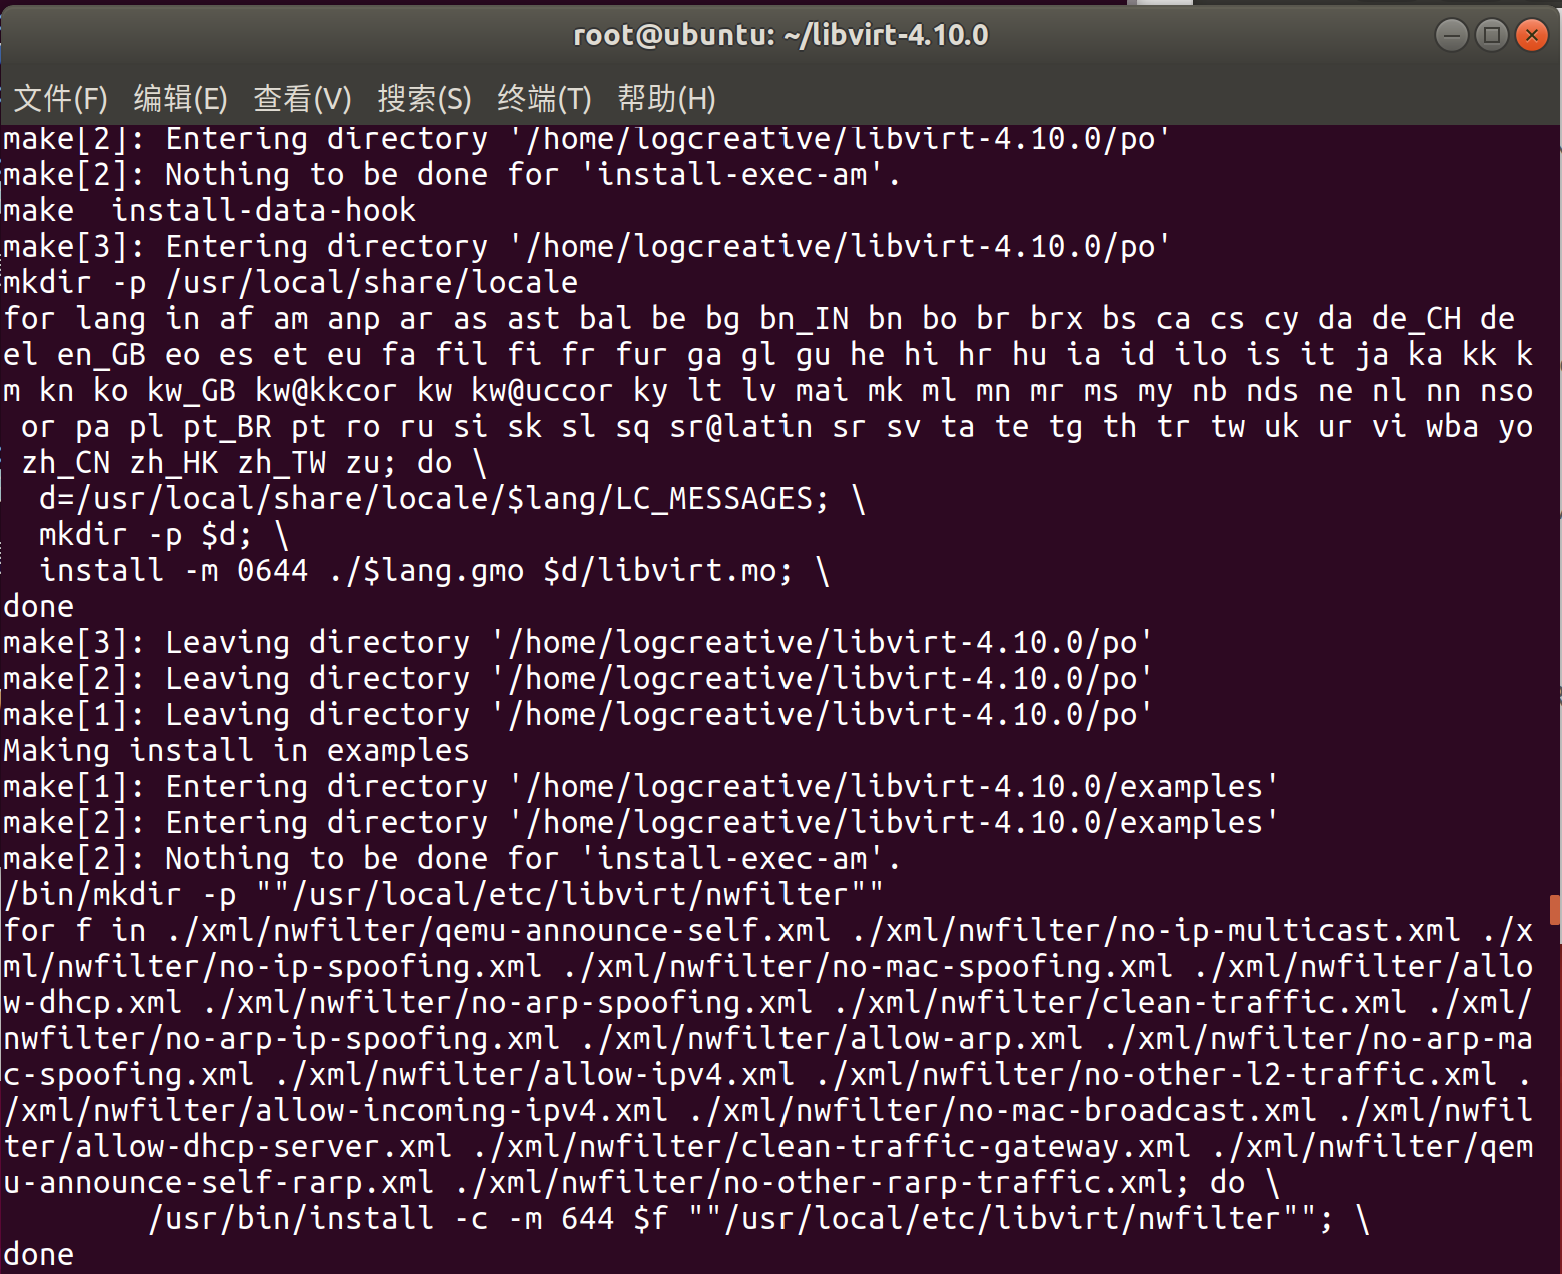
\includegraphics[width=0.95\linewidth]{makelibvirt}
            \caption{编译 libvirt}\label{fig:makelibvirt}
        \end{minipage}
    \end{figure}

    安装完成后,验证 virsh 能够正常启动。之后\textbf{重启系统}以让系统完成一些刷新操作\footnote{不重启系统会导致意想不到的错误。}。

    \begin{figure}[H]
        \centering
        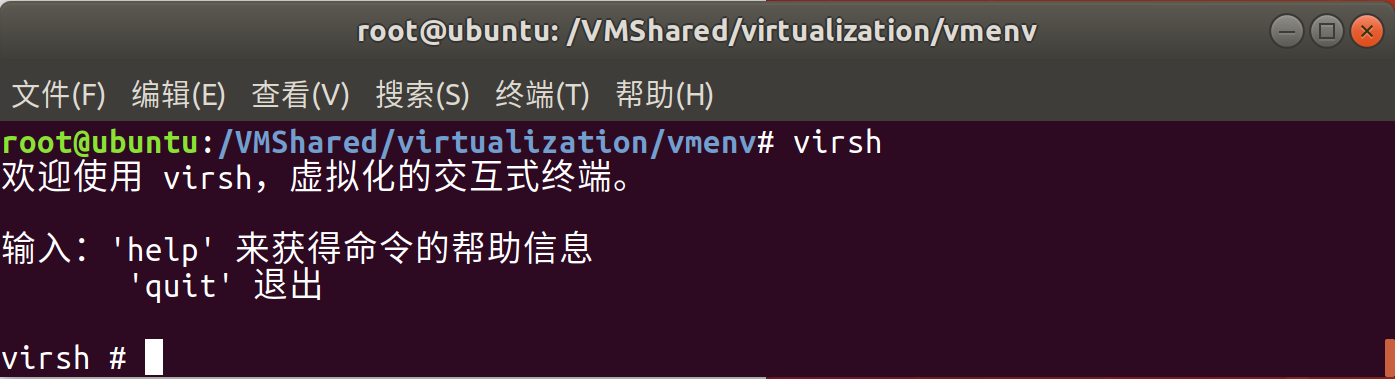
\includegraphics[width=0.95\linewidth]{virsh}
        \caption{运行 virsh 命令}\label{fig:virsh}
    \end{figure}

    \section{注册虚拟机}

    前一次的作业已经使用 QEMU 制作完成了一个虚拟机 \verb"ubuntu.img",使用 \verb"virt-install" 命令安装之(其中\verb"--import"参数用于指定导入现有的磁盘映像),如图 \ref{fig:createvm} 所示。

    \code[language=bash]{attachvm.sh}

    \begin{figure}[H]
        \centering
        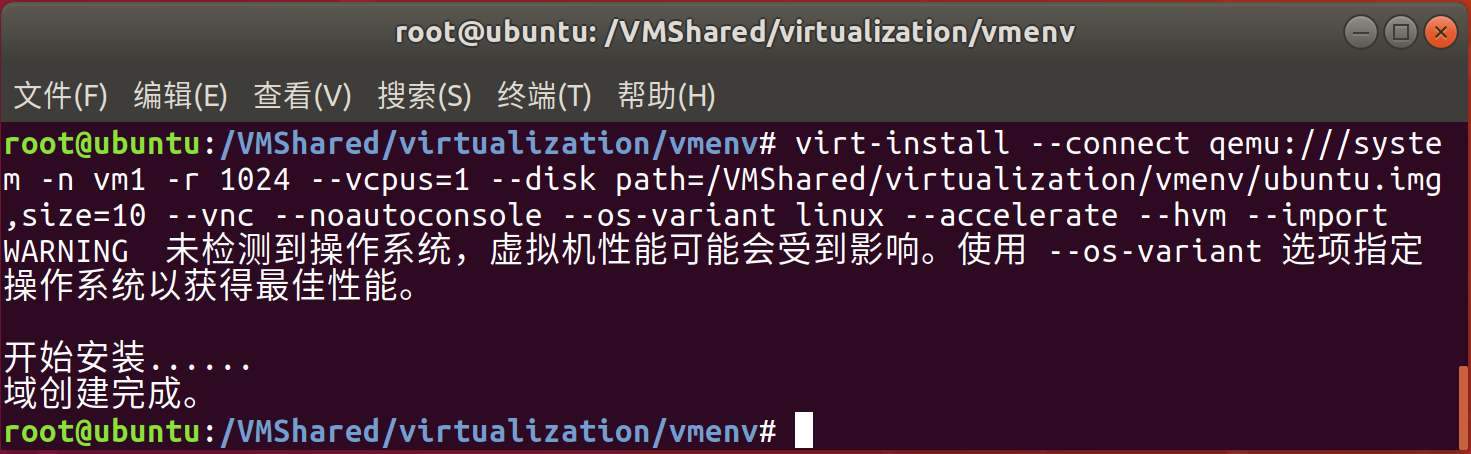
\includegraphics[width=0.9\linewidth]{createvm}
        \caption{注册虚拟机}\label{fig:createvm}
    \end{figure}

    然后使用已经安装好的 \verb"virt-manager" 查看虚拟机状态,如图 \ref{fig:virtmanager}。

    \begin{figure}[H]
        \centering
        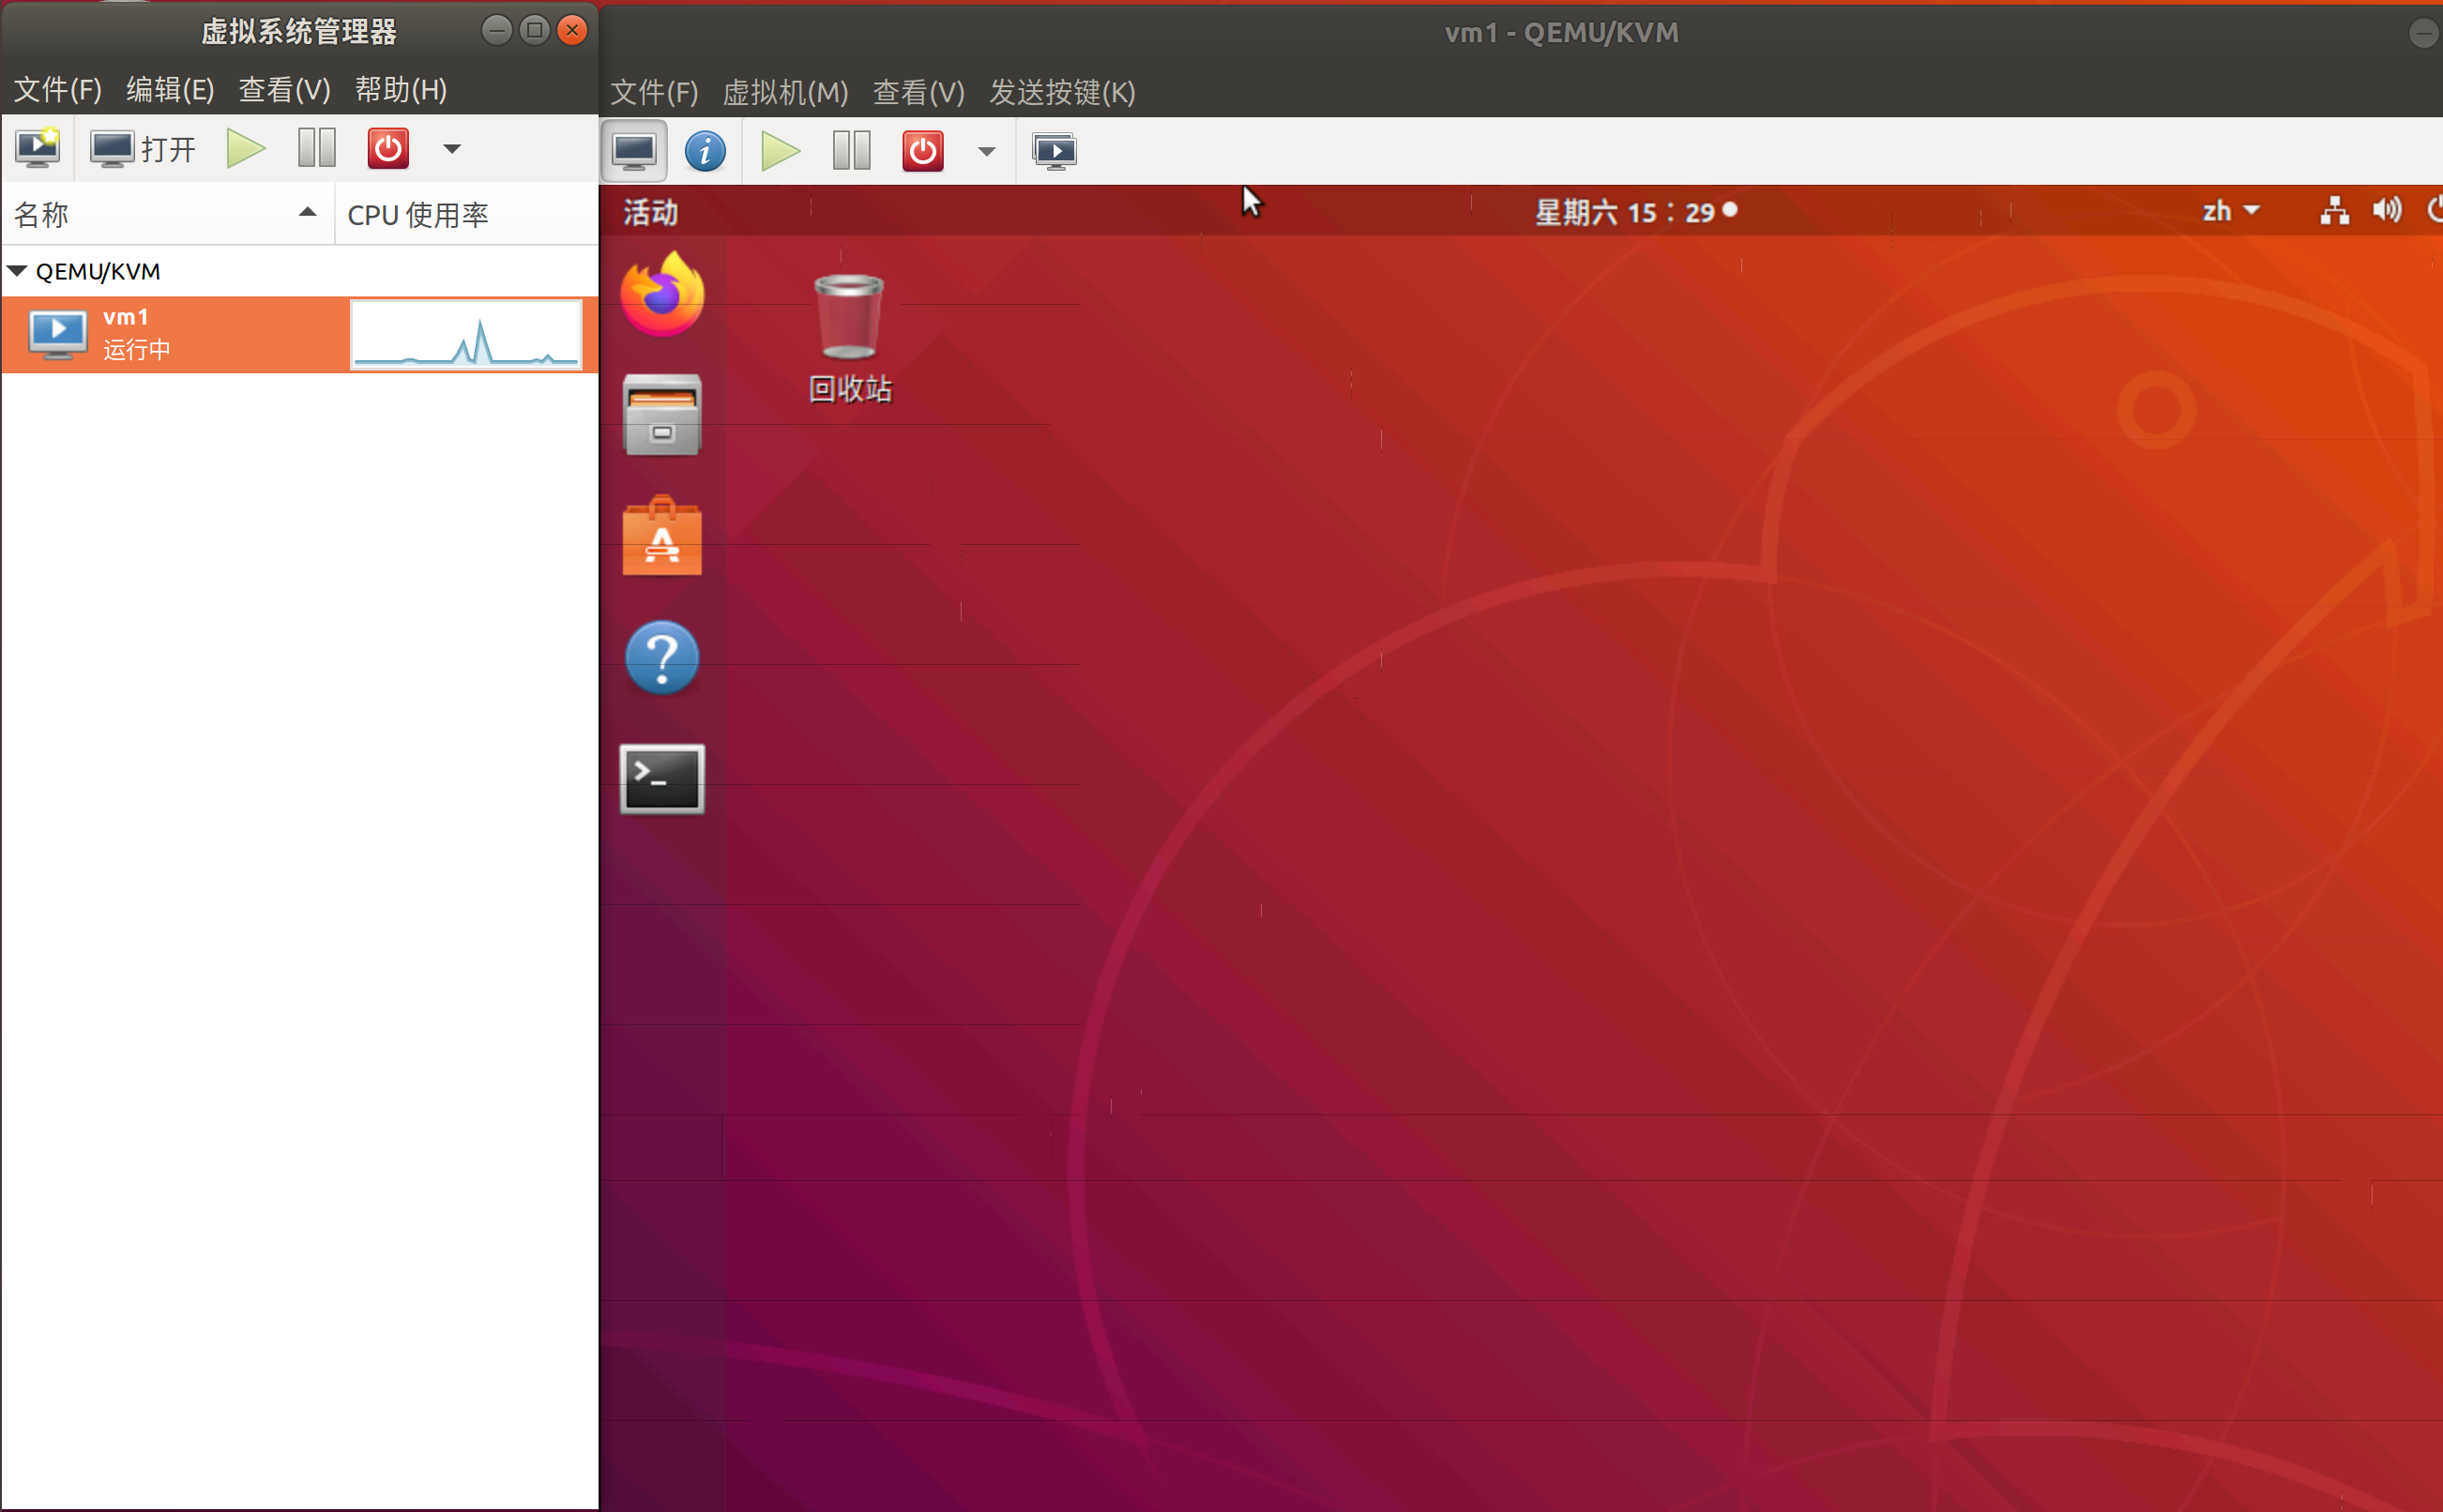
\includegraphics[width=0.9\linewidth]{virtmanager}
        \caption{打开虚拟系统管理器}\label{fig:virtmanager}
    \end{figure}

    \section{获取虚拟机信息}

    通过 libvirt API\cite{libvirtapi},编写下面的 python 脚本获取虚拟机信息。获取结果如图 \ref{fig:getinfo} 所示。

    \code{getvminfo.py}

    \begin{figure}[H]
        \centering
        \includegraphics[width=\linewidth]{getinfo}
        \caption{虚拟机信息}\label{fig:getinfo}
    \end{figure}

    \bibliography{ref}
    
\end{document}